% !TEX spellcheck = en_US
% Tower Damper
%=================================================================================
This section describes the function and the implementation of a pitch angle based \gls{td}. 
The design follows the description in \cite{WindEnergyHandbook} similar as the workflow in the exercise of the corresponding lecture \cite{SchlipfLecture}. 
The tower dynamics are modeled as in \cite{WindEnergyHandbook} (eq: 8.12 and 8.13). 
Here referred to as \ref{eq:TowerDynamics} and \ref{eq:TowerDamper}.
\begin{equation}
	M\ddot{x} + D\dot{x} + Kx = F + \Delta F
	\label{eq:TowerDynamics}
\end{equation}
\begin{equation}
	\begin{aligned}
		\Delta F = \frac{\partial F}{\partial \theta}\Delta\theta = -D_{\text{TD}}\dot{x}\\
		\Delta\theta = \frac{-D_{\text{TD}}}{\partial F/\partial \theta}\dot{x}
	\end{aligned}
	\label{eq:TowerDamper}
\end{equation}
As described by \ref{eq:TowerDynamics} the dynamics of the tower in fore-aft direction are lightly damped if \gls{symb:D} is small and the force $\Delta F$ which is the additional thrust force resulting of a pitch action is equal to zero. The force $F$ is damped by the relative wind speed $v_{\text{rel}} = \gls{symb:v_0} - \dot{x}$ and therefore $F = F(\Omega, \theta, v_{\text{rel}})$ \cite{SchlipfLecture}. To damp the tower top speed \gls{symb:x_dot} even further \cite{WindEnergyHandbook} proposes an update of the pitch angle with $\Delta\theta$. This will damp the tower motion further as described in \ref{eq:TowerDamper}. This leads to a reduction of the tower bottom bending moment. Nevertheless this comes at a cost of higher pitch activity and the damping is only available in control region 3. 
%The static tower top deflection over the regions are shown in section \ref{steady states}. This is helpful to see when the damper is active and what can be damped.

The implementation and test of the damper is done in Matlab and Simulink.
As in the lecture \cite{SchlipfLecture} and corresponding exercise the tower top acceleration \gls{symb:x_dotdot} is used because it is a quantity that is measurable in reality as well.
What is also taken into account is the existence of a real pitch actuator. This means that the pitch update $\Delta\theta$ can not be applied instantaneously because of the time constant of the pitch actuator.
To address this phenomena there are 2 methods tested. 
First a direct integration \ref{eq:TDintegration}: 
\begin{equation}
	\dot{x}(t) = \int\ddot{x}(t) \text{d}t
	\label{eq:TDintegration}
\end{equation} 
And second a phase shift of \SI{90}{\degree} of the acceleration signal by a Lag-Compensator. The transfer function in the frequency domain is shown in \ref{eq:LagCompensator}. Where the input in the frequency domain is $\ddot{X}(s)$ and the output is $\dot{X}(s)$. 
\begin{equation}
	\frac{\ddot{X}(s)}{\dot{X}(s)} = \frac{s + \gls{symb:z}}{s + \gls{symb:p}}
	\label{eq:LagCompensator}
\end{equation} 
\begin{equation}
	\dot{x}(t) = \ddot{x}(t) - \int p\dot{x}(t) - z\ddot{x}(t) \text{d}t
	\label{eq:xddTimeDomain}
\end{equation} 

% explain analytical why this should work better?

The implementation in Simulink (Figure \ref{fig:TDoverview}) is first following the approach in the exercise \cite{SchlipfLecture}.

\begin{figure}[tbh]
	\centering	
	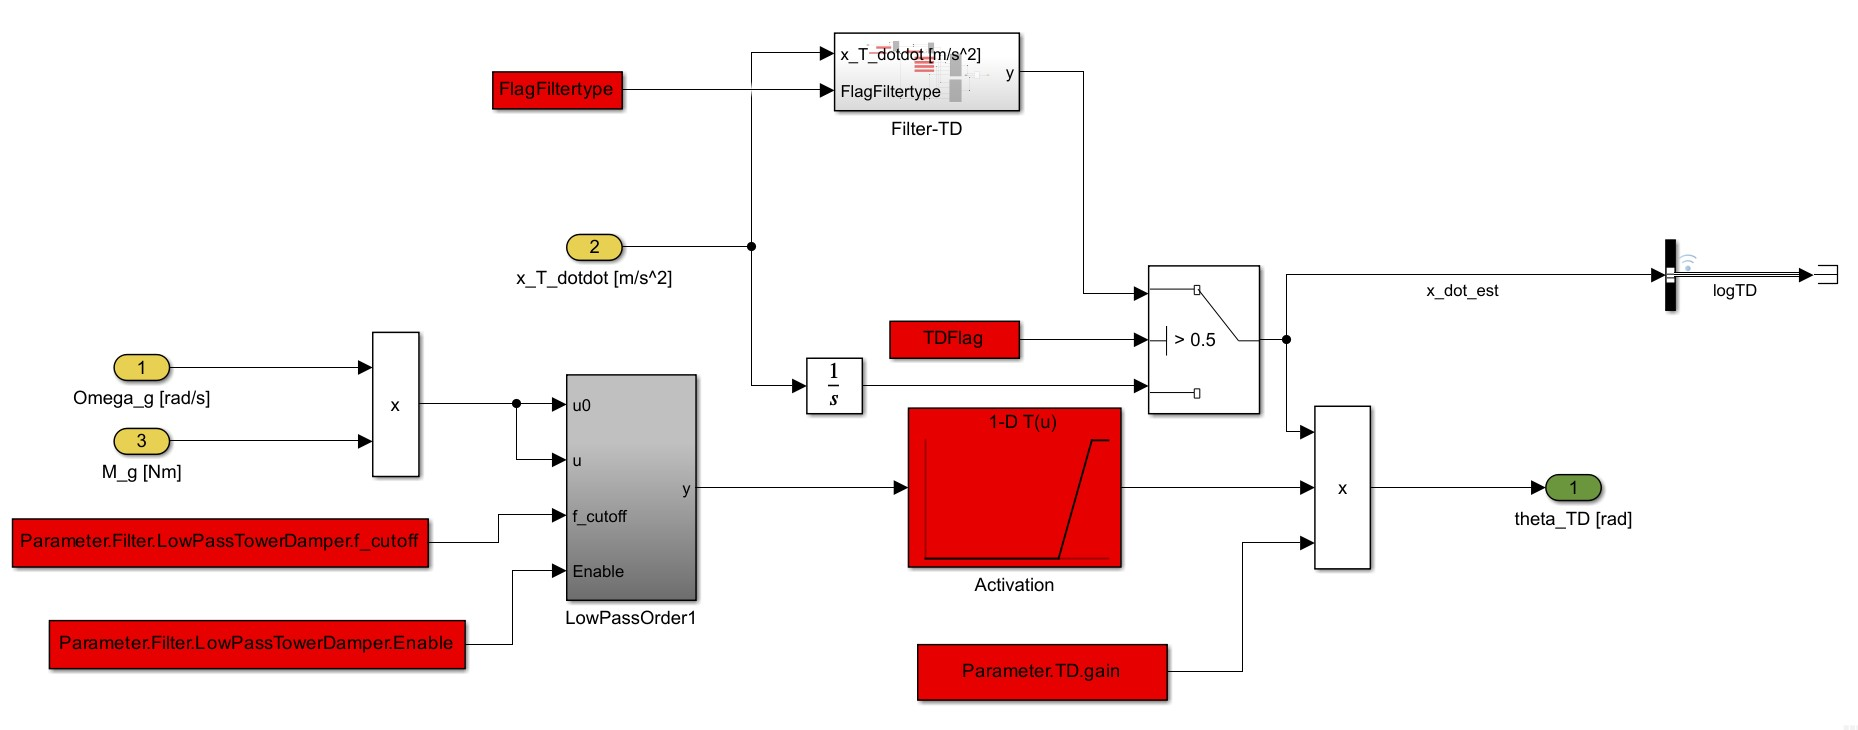
\includegraphics[width=12cm]{Figures/TDoverview}
	\caption{Tower Damper in Simulink model}
	\label{fig:TDoverview}
\end{figure} 

The input \textit{Omega\_g} is already a low pass filtered quantity and the blade passing frequency (3P) is notched out. As shown in Figure \ref{fig:TDoverview} to activate the \gls{td} the generator power is used. The \textit{LowPassOrder1} is used to reduce the switching frequency of the TD to ensure that it is not switched on and off if the \gls{WT} is operating near rated conditions. In the activation the gain is slowly ramped up from $\SI{0}{\%}$ to $\SI{100}{\%}$ over a power range from $\SI{80}{\%}$ of the rated power to $\SI{100}{\%}$.
For higher power values the gain stays at \SI{100}{\%}.

In the first method, here named integrator, the tower top acceleration signal is integrated.
The signal is than multiplied with the damping gain \textit{Parameter.TD.gain} and the activation signal as shown in Figure \ref{fig:TDoverview}.
The resulting quantity is the pitch offset mentioned in \ref{eq:TowerDamper}.
This offset $\Delta\theta$ is added to the pitch angle control value of the \gls{cpc} and this sum is the new input for the SLOW-model. In this first ideal method no pitch actuator is considered.

\begin{figure}[h]
	\centering	
	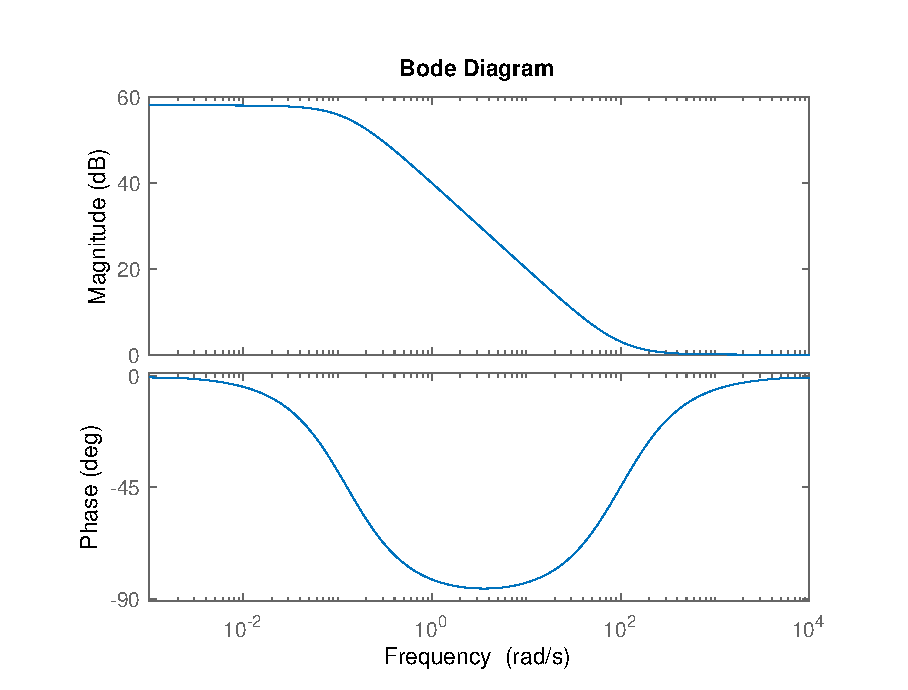
\includegraphics[width=12cm]{Figures/BodeLagCompensator.eps}
	\caption{Bode plot of the Lag-Compensator with tower eigenfrequency (black)}
	\label{fig:BodeLag}
\end{figure}

The second method, here named Lag-Compensator, isolates the tower eigenfrequency by passing the acceleration signal first through a low pass filter and than a high pass filter. The cutoff frequency of both filters is the eigenfrequency of the tower. Now the signal contains mainly the isolated eigenfrequency of the tower with which the tower is oscillating in the fore-aft direction. To phase shift the signal a Lag-Compensator is used. 


As shown in Figure \ref{fig:BodeLag} the frequency is phase shifted by nearly \SI{37}{\degree} and the magnitude is increasing by $\SI{23}{dB}$. This leads with an included pitch actuator that behaves like a PT2-Filter to an overall system shift of \SI{90}{\degree} and a magnitude increase of $\SI{16.5}{dB}$ see Figure \ref{fig:SystemBode}. The higher magnitude is adjusted by a different gain value.

\begin{figure}[h]
	\centering	
	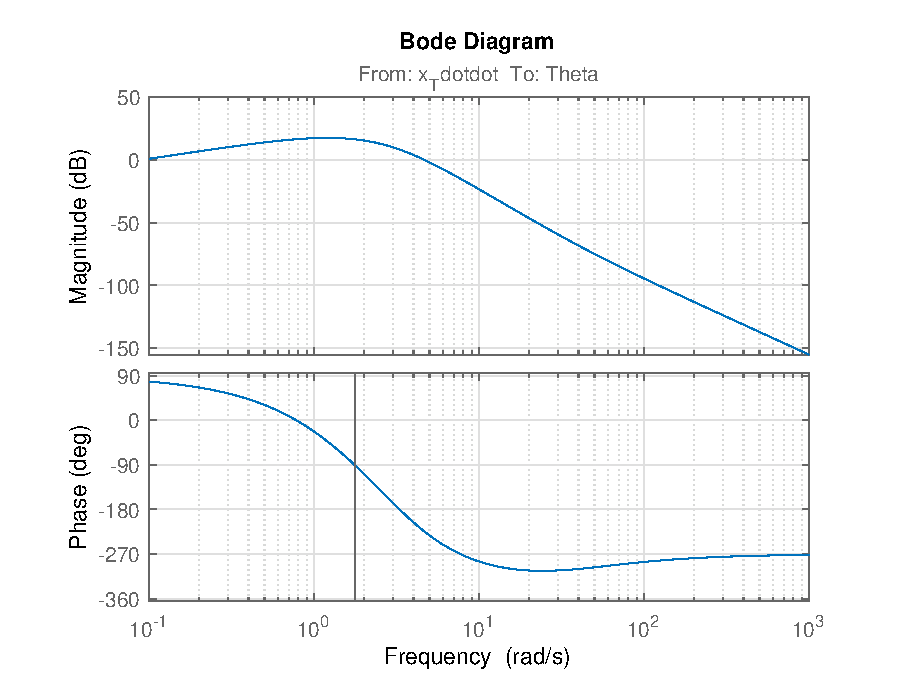
\includegraphics[width=12cm]{Figures/BodeSystem.eps}
	\caption{Bode plot of the Pitch-Actuator and Filter-Chain with tower eigenfrequency (black)}
	\label{fig:SystemBode}
\end{figure} 


The design is tested with a wind step from $v_0 = \SI{20}{m/s}$ to $v_1 = \SI{21}{m/s}$. The results are shown in Figure \ref{fig:TDWindStep}.

\begin{figure}[h]
	\centering	
	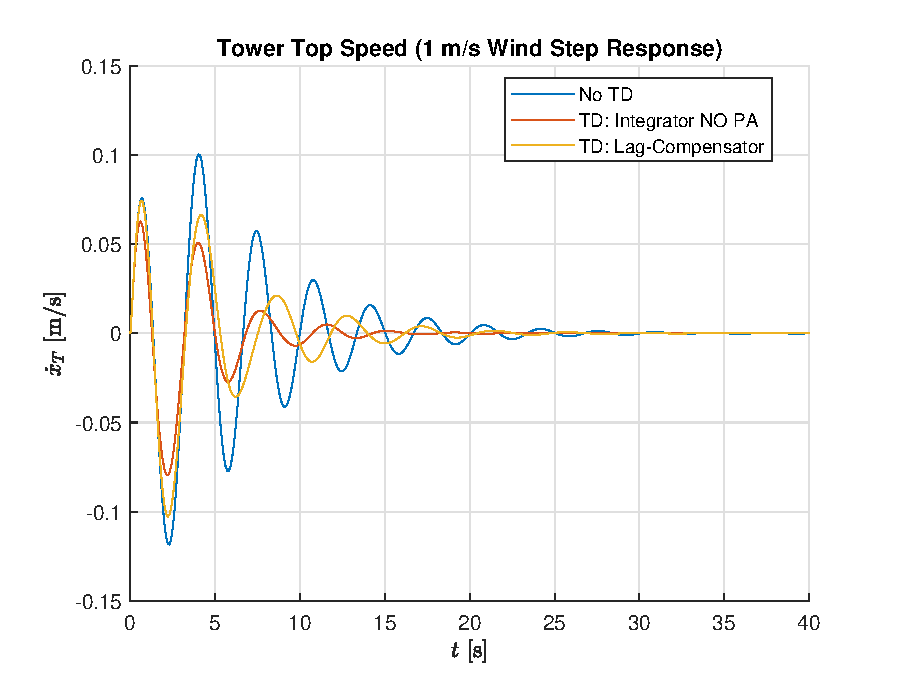
\includegraphics[width=12cm]{Figures/WindStep.eps}
	\caption{Tower-Top-Speed}
	\label{fig:TDWindStep}
\end{figure}

As shown in Figure \ref{fig:TDWindStep} the result is not matching the design and expectations above. 
The tower top speed is not in phase with the integrator method. It is to expect, that the implementation is containing an error.
To debug the system the filter and the integrator method are disturbed by a $\cos$-signal with the eigenfrequency of the tower as shown in Figure \ref{fig:Debug}. 
The two methods are not perfectly aligned. 
The difference at the beginning is not the problem but that the signals are not converting into the same is causing the issue. 
First fine tuning iterations of the Lag-Compensator does not lead to a successful result. 
This issue remains unsolved by the end of the project end requires a deeper investigation. 
 
\begin{figure}[h]
	\centering	
	\includegraphics[width=12cm]{Figures/Debugging.eps}
	\caption{Debugging of the \gls{td} with Lag-Compensator}
	\label{fig:Debug}
\end{figure}
  
The expected result with the filter is, that the loads at the eigenfrequency of the tower are reduced the same way as they are with an integrator.
But due to the fact that the filter is considering the signal delay by the pitch actuator the loads around the eigenfrequency are not increased as with a pure integrator.    